\documentclass[fleqn, 12pt]{SelfArx}
\usepackage[utf8]{inputenc}
\usepackage[T1]{fontenc}
\usepackage[italian]{babel}
\usepackage{lmodern}
\usepackage{csquotes}
\usepackage{subcaption}
\usepackage{graphicx}
\usepackage{biblatex}

\setlength{\columnsep}{0.55cm} % Distance between the two columns of text
\setlength{\fboxrule}{0.75pt} % Width of the border around the abstract

\definecolor{color1}{RGB}{0,0,90} % Color of the article title and sections
\definecolor{color2}{RGB}{0,20,20} % Color of the boxes behind the abstract and headings

\usepackage{hyperref} % Required for hyperlinks

\hypersetup{
	hidelinks,
	colorlinks,
	breaklinks=true,
	urlcolor=color2,
	citecolor=color1,
	linkcolor=color1,
	bookmarksopen=false,
	pdftitle={Smart Box IoT},
	pdfauthor={Lorenzo Calisti},
}

\addbibresource{relazione.bib}

\JournalInfo{Programmazione per l'IoT - Laurea Magistrale in Informatica Applicata - DiSPeA - Università degli Studi di Urbino Carlo Bo} % Journal information
\Archive{Data di pubblicazione xx/xx/xxxx - DOI: xxxx/xxxxxxx} % Informazioni che verranno inserite dal Docente in fase di pubblicazione

\PaperTitle{Smart Box IoT} % Article title

\Authors{Lorenzo Calisti\textsuperscript{1}*, Emanuele Lattanzi\textsuperscript{2}} % Il docente Emanuele Lattanzi figura come autore
% al fine di poter gestire la procedura di submission sul repository pubblico (nell'affiliazione viene chiarito il ruolo)
\affiliation{\textsuperscript{1}\textit{Laurea Magistrale in Informatica Applicata, Università degli Studi di Urbino Carlo Bo, Urbino, Italia}} % Author affiliation
\affiliation{\textsuperscript{2}\textit{Docente di Programmazione per l'Internet of Things, Università degli Studi di Urbino Carlo Bo, Urbino, Italia}} % Author affiliation
\affiliation{*\textbf{Corresponding author}: l.calisti@campus.uniurb.it} % Corresponding author

\Keywords{Internet of Things --- Machine Learning --- Arduino --- ESP8266 --- Anomaly Detection} % Keywords - if you don't want any simply remove all the text between the curly brackets
\newcommand{\keywordname}{Keywords} % Defines the keywords heading name

\Abstract{
Negli ultimi anni il tema del cambiamento climatico e delle sue conseguenze è sempre più presente nelle menti della popolazione; secondo gli esperti è fondamentale che tutti i settori produttivi si impegnino sin 
da subito ad utilizzare energie rinnovabili e a creare nuovi metodi produttivi in modo da ridurre le emissioni. Per fare questo si prevede un ampio utilizzo della tecnologia, in particolare dell'Internet of Things.
Il campo dell'agricoltura è uno dei settori pionieri da questo punto di vista; è ormai da diverso tempo che la tecnologia è utilizzata come supporto alla produzione, il principale problema è il suo elevato costo 
che la rende accessibile solo ad aziende di grandi dimensioni.
In questo articolo si propone la creazione di una Smart Box IoT la cui finalità principale è la raccolta di dati sulla qualità dell'ambiente circostante e il rilevamento di eventauali dati anomali tramite 
un modello di Machine Learning.}

\begin{document}

\maketitle

\section{Introduzione}

In questi anni si sente sempre più parlare della minaccia del cambiamento climatico e di come esso affliggerà le vite di tutta la popolazione in un futuro non troppo lontano, per questo motivo è fondamentale 
un cambio di mentalità da parte di tutte le industrie volto all'utilizzo di energie rinnovabili e alla creazione di nuovi metodi produttivi in modo di ridurre i consumi, le emissioni e l'inquinamento globale.

Secondo i maggiori esperti la tecnologia avrà un impatto decisivo nella vittoria di questa "guerra"; il suo ruolo è quello di supporto, ottimizzando i vecchi processi produttivi
e aiutando nella scoperta di nuovi metodi di produzione più eco sostenibili con meno sprechi e consumi.
Nel campo dell'agricoltura l'utilizzo della tecnologia come supporto alla produzione sta prendendo piede ormai da diversi anni, il problema principale è l'elevato costo che la rende accessibile solo ad aziende di grandi dimensioni.

Il tipo di tecnologia più comune in ambiente agricolo è la "centralina meteo" posizionata nei campi che consente di raccogliere continuamente dati sulle attuali condizioni atmosferiche e sulla qualità del terreno in modo
da sapere quale sia il miglior momento per irrigare, riducendo lo spreco d'acqua, capire se è arrivato il momento del raccolto, evitando la raccolta di prodotti non ancora pronti, e addirittura prevedere piogge o 
periodi di siccità futuri, in modo da prepararsi preventivamente ad essi.

La raccolta passiva dei dati è un tipo di tecnologia utilizzato dalle grandi industrie da più di quarant'anni, il vero elemento innovativo è l'utilizzo dell'IoT. L'internet of things\cite{iot}, IoT in breve, rappresenta l'unione del
mondo reale, le cose, con il mondo virtuale, la rete internet; il suo scopo è quello di connettere fra loro tutti i sistemi fisici di raccolta dei dati dandogli un "cervello". Citando il creatore dell'IoT Kevin Ashton: 

\begin{displayquote}
  In the twentieth century, computers were brains without senses - they only knew what we told them. In the twenty-first century, because of the Internet of Things, computer can sense things for themselves
\end{displayquote}

La "Smart Box" IoT creata in questo articolo tiene bene a mente tutte queste idee; la sua funzionalità principale è quella di raccogliere dati sulla qualità dell'ambiente circostante in maniera continuativa per poi 
elaborarli "sul posto" e rilevare eventuali anomalie che sono poi segnalate ad un sistema di monitoraggio remoto. Per fare questo si è partiti dalla progettazione e realizzazione del'hardware, per poi passare alla raccolta
dei dati "raw" e finire con l'addestramento di un modello di Machine Learning in grado di rilevare le anomalie dai dati che è poi stato installato nella Smart Box.
Di seguito vedremo più nel dettaglio tutte queste fasi con l'aggiunta di un analisi statistica sui dati raccolti inizialmente e sulle anomalie rilevate.

\section{Progettazione Smart Box}

La "Smart Box" IoT, come dice il suo nome, è una scatola intelligente, con al suo interno una serie di sensori e un MCU impostati per raccogliere i dati una volta ogni 15 minuti. L'intera scatola è stata progettata 
per essere montata su un supporto in modo da rimanere sempre sollevata dal terreno, il che è l'ideale per l'installazione in un campo dove, con la crescita delle colture, rischia di non essere più del tutto visibile.

Vediamo ora nel dettaglio tutti i componenti presenti all'interno della "Smart Box". Il più importante è senza dubbio l'MCU ESP8266, è il cuore dell'intero sistema, un chip a basso costo con Wi-Fi integrato e diversi pin
GPIO, molto popolare nelle applicazioni IoT.
Nella "Smart Box" sono stati inseriti i seguenti sensori:

\begin{itemize}
\item DHT11, sensore di temperatura e umidità
\item Sensore di rilevamento della pioggia 
\item YL-69, sensore igrometro per il rilevamento dell'umidità del terreno
\item MQ-135, sensore per il monitoraggio della qualità dell'aria
\item LDR, sensore di luminosità 
\item BMP180, sensore combinato di temperatura, pressione e altitudine
\end{itemize}

Oltre a questi componenti all'interno della scatola è stato inserito anche un LED di colore giallo utilizzato per segnalare lo stato del programma ed eventuali errori; infine, per alimentare l'MCU e tutti i sensori si 
è optato per la soluzione più semplice: un power-bank portatile con uscita a 5V, in questo modo non solo si evitano i diversi problemi dovuti alla gestione delle batterie LiPo, ma anche la ricarica è più 
facile e sicura, utilizzando un semplice caricatore per smartphone.

Una volta scelti tutti i componenti il primo passo per la progettazione della Smart Box è quello di realizzare delle schematiche che mostrino i diversi collegamenti elettrici fra loro; la Figura \ref{fig:schematics} 
e la Figura \ref{fig:breadboard} mostrano proprio questi schemi che sono stati fondamentali durante la fase di costruzione per tenere traccia di tutti i collegamenti elettrici. Questi diagrammi sono stati realizzati 
utilizzando Fritzing\cite{fritzing}: un programma open source per la progettazione di schemi elettrici.

\begin{figure}[htb]
\centering
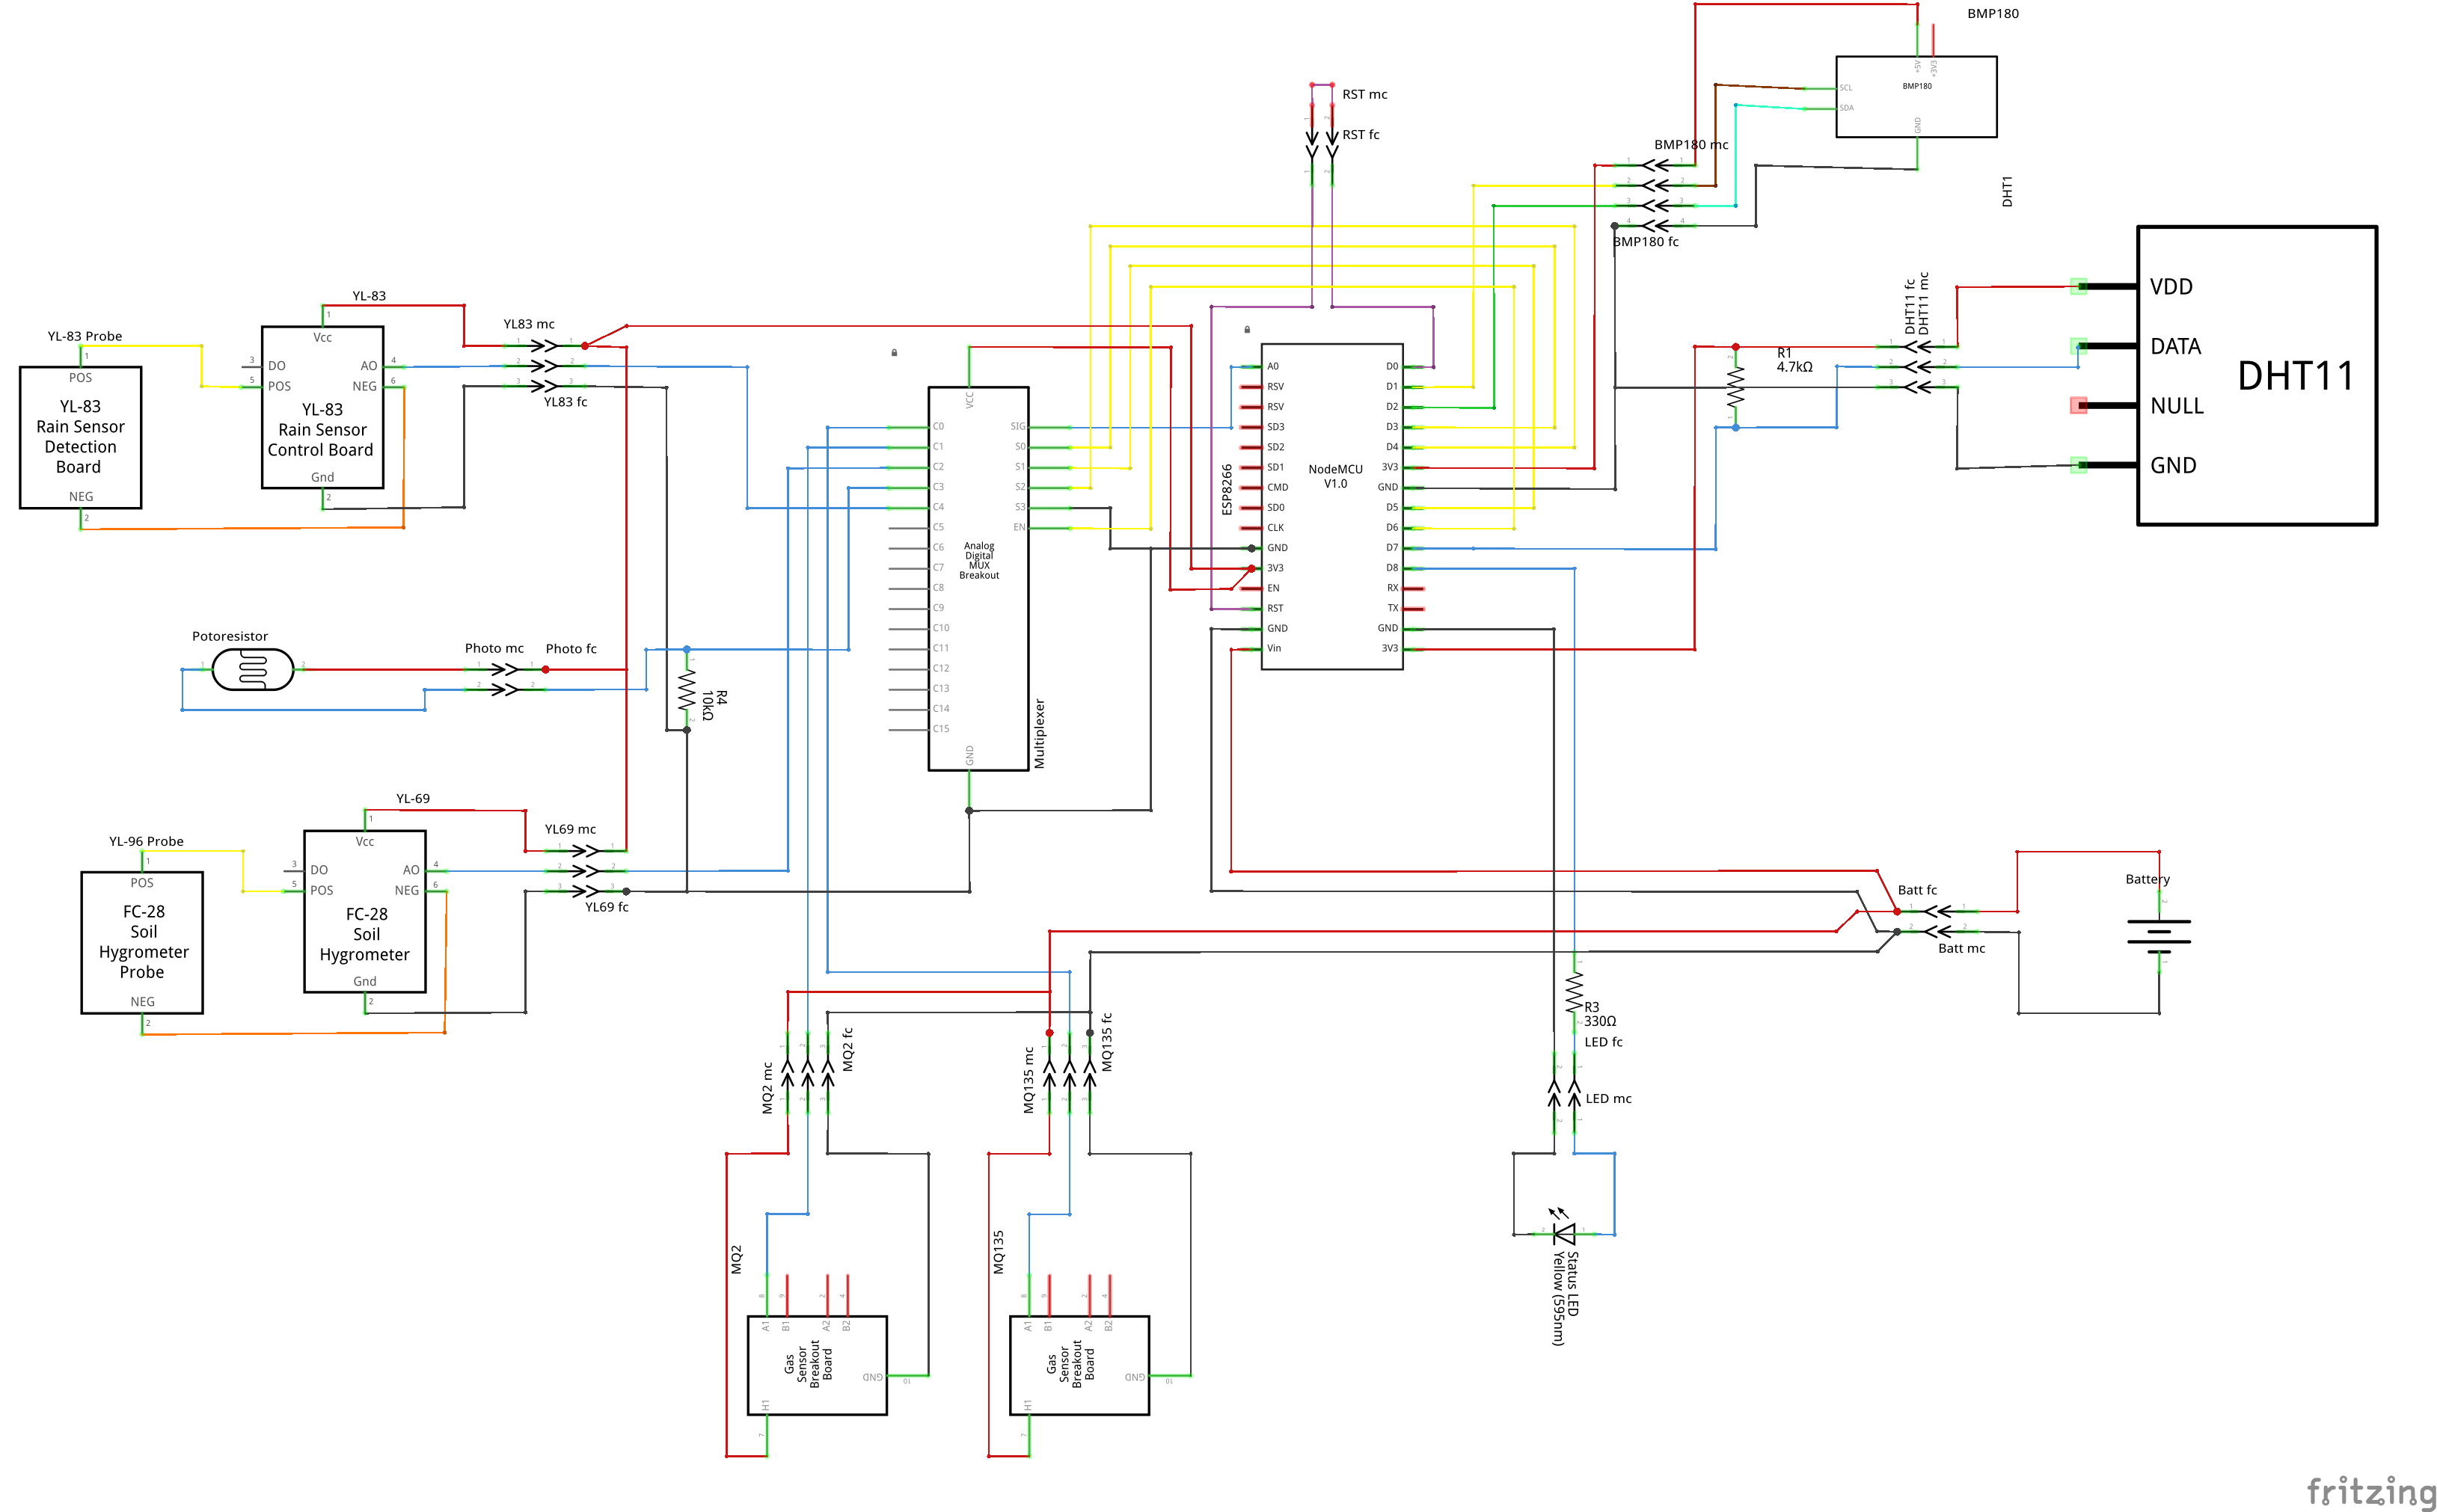
\includegraphics[scale=0.25]{hardware/iot_project_schem.png}
\caption{Schematica del circuito}
\label{fig:schematics}
\end{figure}

\begin{figure}[htb]
\centering
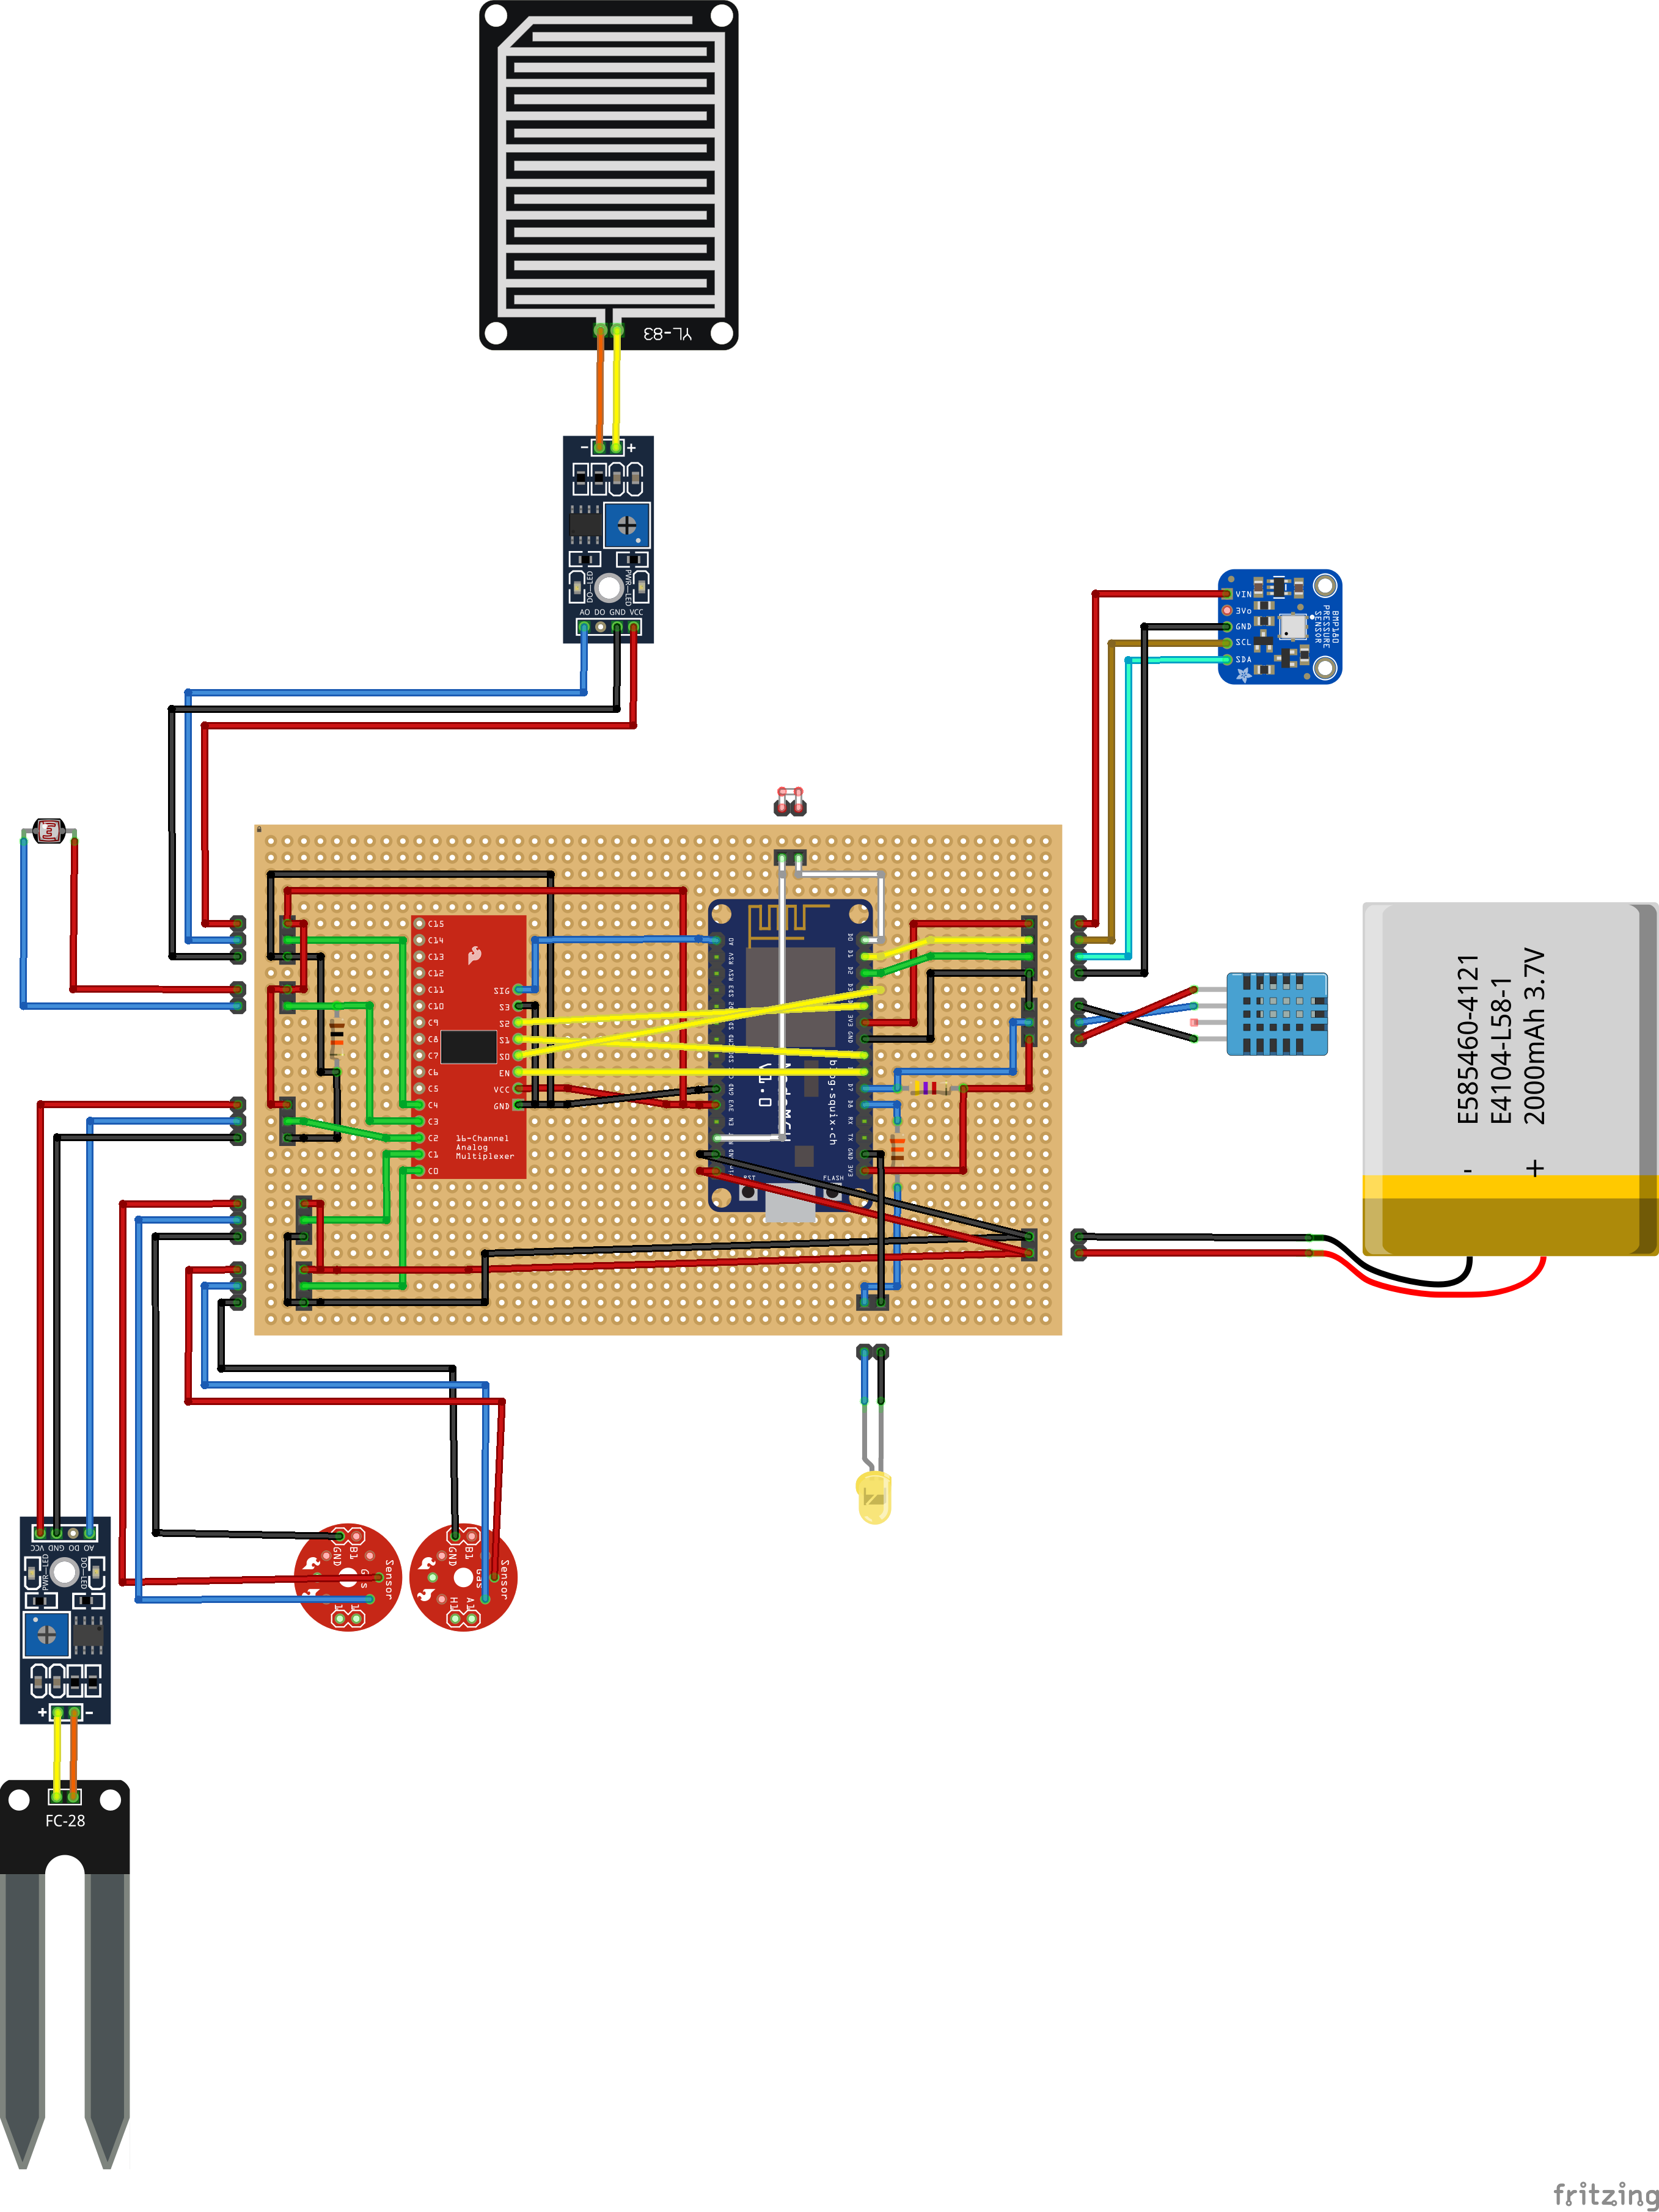
\includegraphics[scale=0.25]{hardware/iot_project_bb.png}
\caption{Schematica della breadboard}
\label{fig:breadboard}
\end{figure}

\begin{figure}[htb]
  \centering
  \subcaptionbox{Vista della scatola}{\includegraphics[scale=0.25]{hardware/smart_box.pdf}}
  \subcaptionbox{Vista della scatola + supporto}{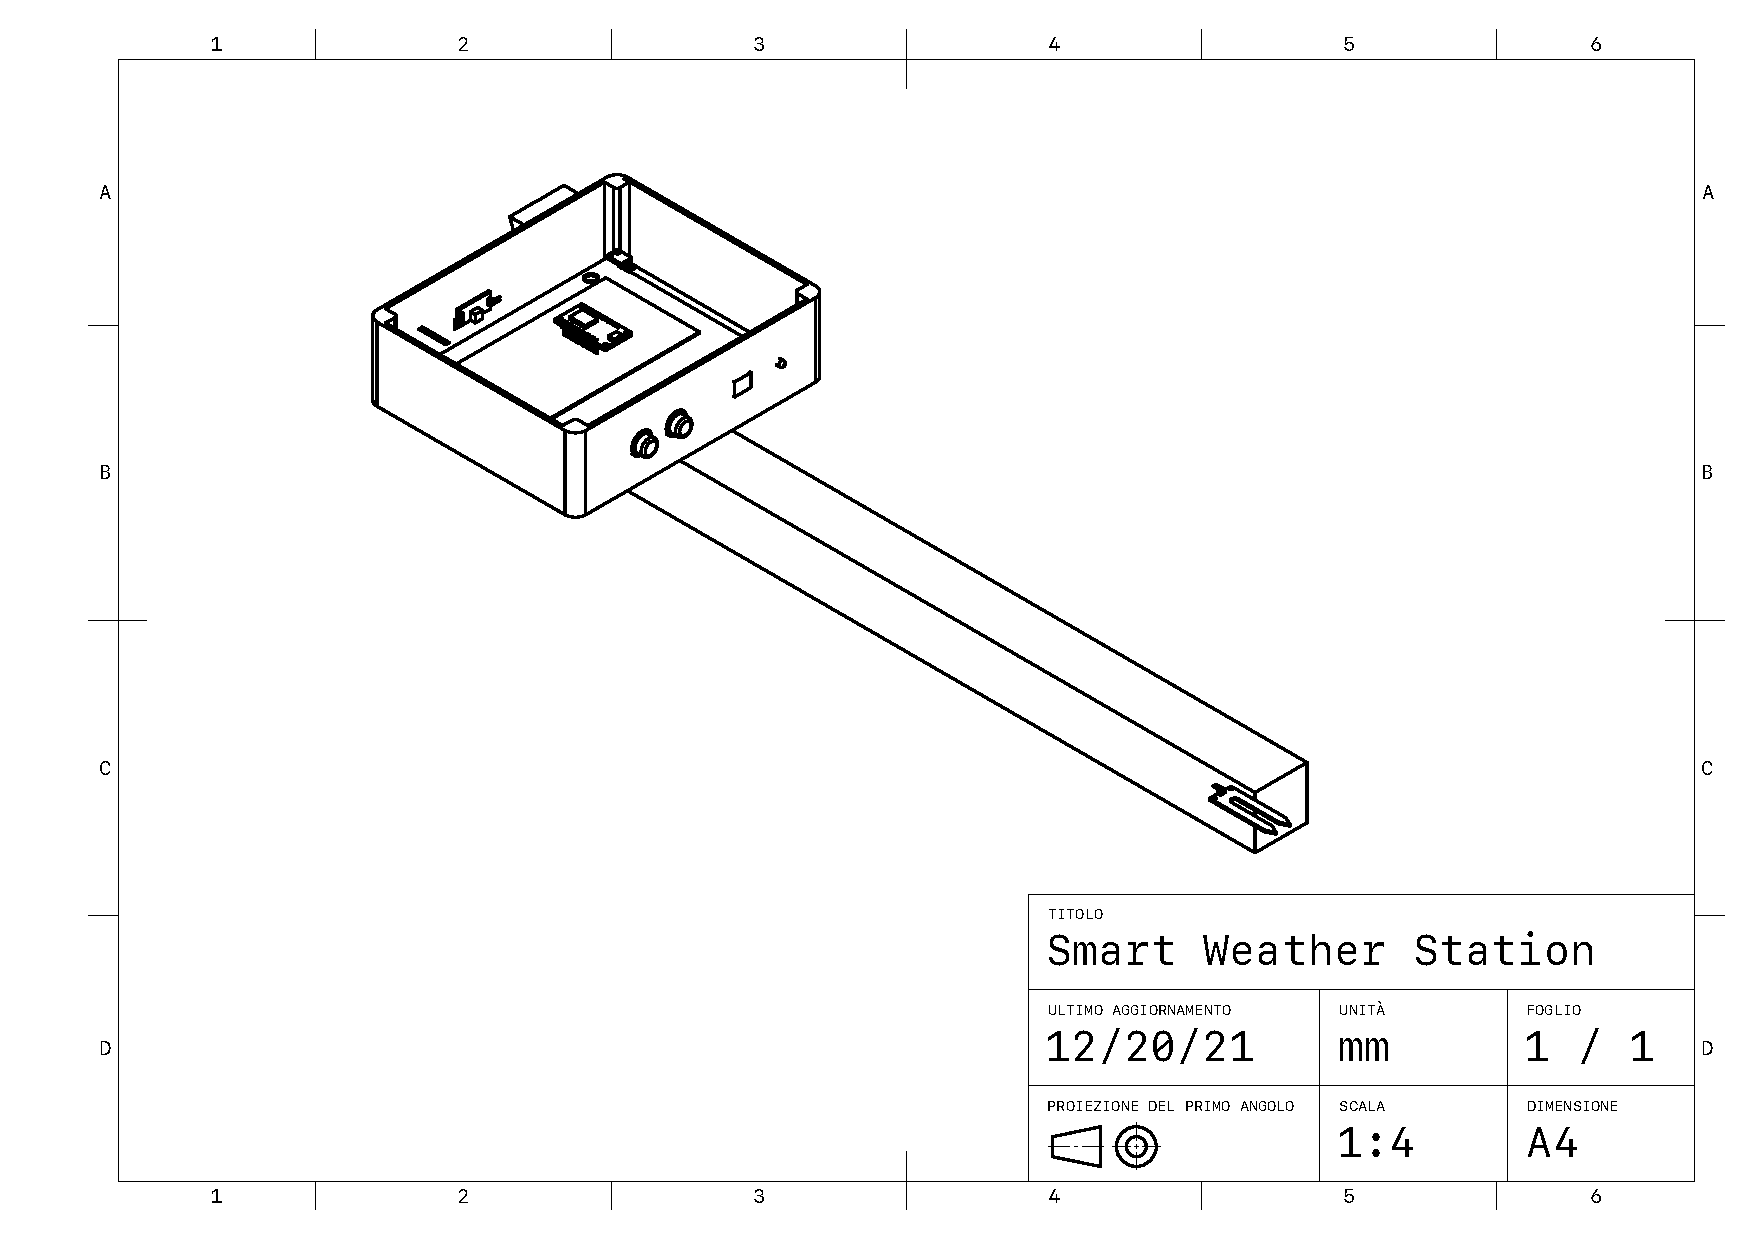
\includegraphics[scale=0.25]{hardware/smart_box_complete.pdf}}
  \caption{Modelli 3D della Smart Box}
  \label{fig:models}
\end{figure}

In aggiunta a questi due schemi è stato anche realizzato un modello 3D di tutti i componenti, compresa la scatola che li racchiude, per essere sicuri delle loro misure effettive; 
i disegni in Figura \ref{fig:models} sono stati creati utilizzando lo strumento per la progettazione di modelli 3D Shapr3D\cite{shapr3d}. 

Una volta progettata la Smart Box si è passati alla fase di realizzazione: acquistati i diversi componenti gli schemi sono stati assemblati su una base mille-fori ottenendo il risultato in Figura \ref{fig:assembled}.

\begin{figure}[htb]
\centering
\includegraphics[scale=0.05]{assets/IMG_20220126_105605.jpg}
\caption{Circuito realizzato su breadboard}
\label{fig:assembled}
\end{figure}

\section{Raccolta dei dati}

Per la raccolta dei dati generati dai sensori si è deciso di scrivere un programma utilizzando Arduino\cite{arduino}, popolare piattaforma open source per lo sviluppo di programmi eseguibili su micro-controllori, poiché 
integra nativamente tutte le librerie necessarie per interagire con i sensori e con l'ESP8266. 

Il programma, chiamato `collector.ino`, si connette alla rete WiFi preconfigurata ad ogni avvio dell'MCU, raccoglie i dati provenienti da ogni sensore in quell'instante di tempo e li invia ad un server InfluxDB\cite{influxdb} 
etichettati in maniera appropriata, infine sfrutta la funzionalità di Deep Sleep dell'ESP8266 per mandare l'MCU in uno stato di sonno profondo per altri 15 minuti. In questo modo sia L'ESP che i sensori sono 
disattivati completamente (a parte un circuito interno all'ESP usato per il risveglio) riducendo al minimo il consumo di corrente.

Come detto precedentemente i dati raccolti dalla Smart Box sono caricati sul cloud utilizzando il servizio InfluxBD, un database open-source per serie temporali che offre strumenti di raccolta e analisi appositamente 
creati per gestire questo tipo di dato molto comune nell'ambiente IoT.

\begin{figure}[htb]
\centering
\includegraphics[scale=0.05]{assets/IMG_20211222_112505.jpg}
\caption{Smart Box nella sua posizione finale}
\label{fig:inplace}
\end{figure}

Una volta realizzata la Smart Box si è deciso di posizionarla in una parte di giardino adibita ad orto nelle vicinanze di casa mia, Figura \ref{fig:inplace}, questo posto è perfetto poiché è molto simile ad un campo agricolo, 
inoltre è abbastanza vicino da collegarsi alla rete WiFi di casa senza aver bisogno di particolari antenne per estendere il segnale. 
Una volta nella sua posizione definitiva la raccolta dei dati può aver inizio; il periodo di raccolta va dal giorno 23/12/2021 al giorno 17/01/2022, per un totale di 25 giorni che, con la frequenza di un campione 
ogni 15 minuti, ha prodotto all'incirca 2400 campioni singoli.

\section{Analisi dei dati}

\begin{table*}[htb]
  \centering
  \begin{tabular}{ l l l l l }
    \hline
    & media & std & mediana & moda (n.) \\
    \hline
    temperatura DHT11 & 6.17 & 4.69 & 6.0 & 4.0 (216) \\
    temperatura BMP180 & 5.87 & 6.29 & 4.9 & 4.5 (29) \\
    umidità & 83.87 & 9.72 & 87.0 & 88.0 (856) \\
    LDR\% & 38.08 & 46.91 & 0.0 & 0.0 (1319) \\
    pioggia\% & 14.13 & 28.41 & 1.0 & 1.0 (1754) \\
    igrometro\% & 53.42 & 15.81 & 57.0 & 58.0 (187) \\
    MQ-135\% & 8.32 & 1.65 & 8.0 & 8.0 (1672) \\
    pressione & 96357.00 & 845.43 & 96376.0 & 95411.0 (6) \\
    altitudine & 423.11 & 73.31 & 421.21 & 354.49 (7) \\
    \hline
  \end{tabular}
  \caption{ Valori statistici ricavati da ogni sensore }
  \label{tab:all_data_stats}
\end{table*}

I dati raccolti sono stati elaborati in parte utilizzando il sistema di query nativo di InfluxDB\cite{flux} ed in parte con uno script python\cite{python}.

Guardando la Tabella \ref{tab:all_data_stats} possiamo vedere diversi fenomeni interessanti: innanzitutto la temperatura media rilevata dal sensore DHT11 e quella rilevata da BMP180 sono molto simili, 
questo ci da conferma del corretto funzionamento dei due sensori. Come seconda cosa notiamo che la media del sensore LDR è del 38\% poiché, essendo inverno durante il periodo di raccolta dati, 
ci sono state più ore di buio che di luce. Analizzando il sensore di gas MQ-135 si nota che il suo valore medio, mediano e modale è all'incirca di 8\%, con una variazione del 1.6\%, questo indica 
che durante l'intero periodo di misurazione la qualità dell'aria è rimasta sempre all'incirca costante. Se confrontiamo i valori ricavati dal sensore di pioggia con quelli dell'igrometro possiamo vedere 
come il valore medio della pioggia sia del \textasciitilde14\%, mentre il valore dell'igrometro del
\textasciitilde53\% indicando che durante il periodo di misurazione ci sono state poche precipitazioni ed il terreno è rimasto mediamente umido. Infine vediamo che la percentuale media dell'umidità è 
del 83\% con una deviazione standard del \textasciitilde9\% ovvero durante l'intero periodo di misurazione l'umidità è rimasta pressoché costante.

\begin{figure}[htb]
  \centering
  \subcaptionbox{sensori di temperatura DHT11 e BMP180}{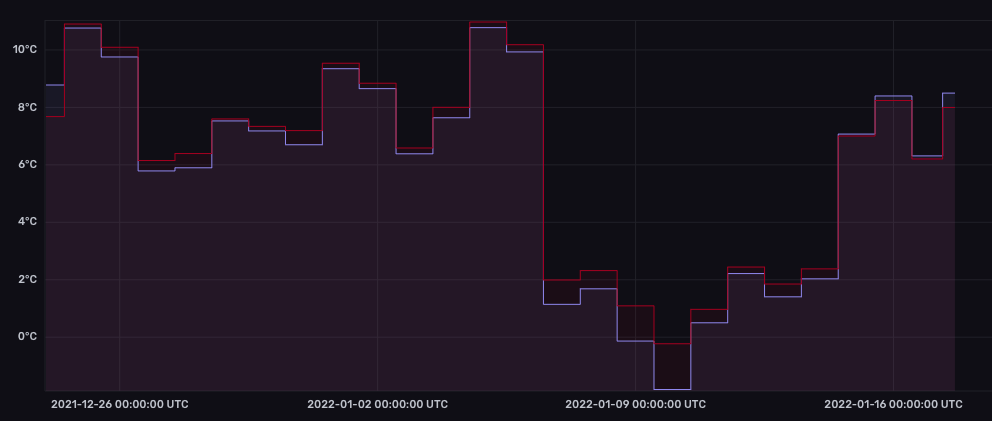
\includegraphics[scale=0.22]{assets/mean_dht_bmp_temp.png}}
  \subcaptionbox{sensore umidità}{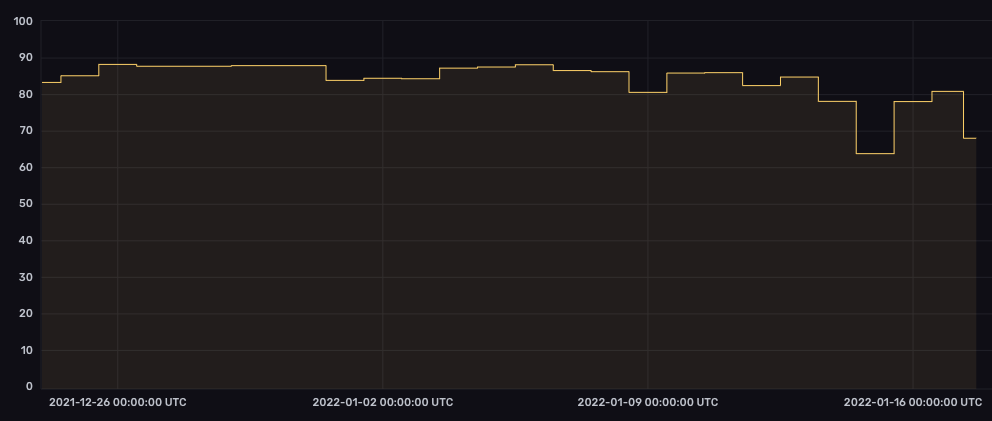
\includegraphics[scale=0.22]{assets/mean_hum.png}}
  \subcaptionbox{sensore LDR}{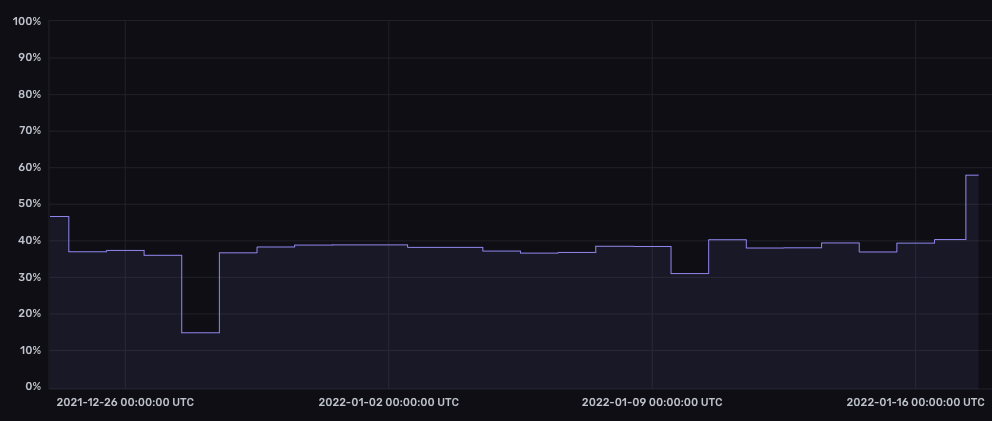
\includegraphics[scale=0.22]{assets/mean_ldr.png}}
  \subcaptionbox{sensori di pioggia e igrometro}{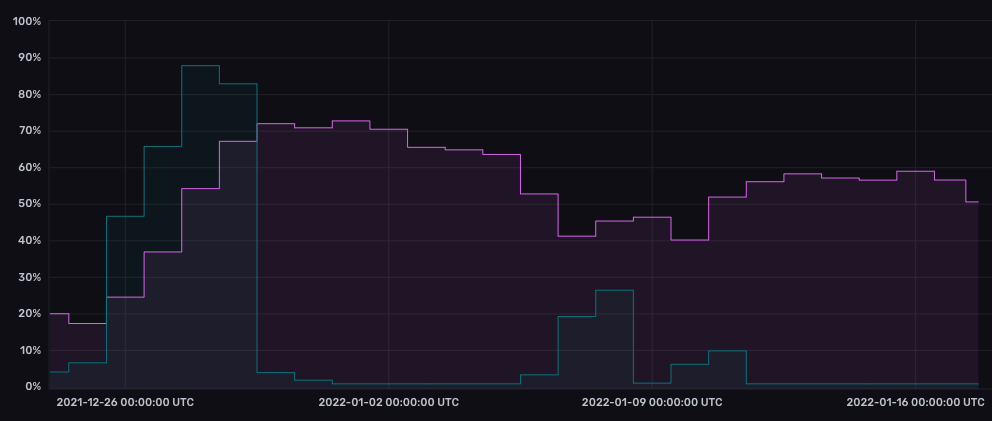
\includegraphics[scale=0.22]{assets/mean_igro_rain.png}}
  \caption{Grafici con le medie giornaliere di alcuni sensori}
  \label{fig:plots}
\end{figure}

Nella Figura \ref{fig:plots} possiamo vedere alcuni grafici ottenuti applicando una finestra di un giorno ai dati e calcolando la media al suo interno facendola poi scorrere fino alla fine.

\begin{table*}[htb]
  \centering
  \begin{tabular}{ l l l l l }
    \hline
    & media giorno & media notte & min/max giorno & min/max notte \\
    \hline
    temperatura DHT11 & 8.71 & 4.55 & -1.0/26.0 & -3.0/13.0 \\
    temperatura BMP180 & 9.90 & 3.31 & -3.9/31.0 & -4.9/11.8 \\
    umidità & 80.08 & 86.27 & 29.0/91.0 & 49.0/91.0 \\
    pioggia\% & 11.85 & 15.57 & 1.0/96.0 & 1.0/95.0 \\
    igrometro\% & 53.50 & 53.37 & 1.0/84.0 & 16.0/74.0 \\
    LDR\% & 96.29 & 1.14 & 50.0/100.0 & 0.0/49.0 \\
    MQ-135\% & 8.42 & 8.26 & 3.0/66.0 & 3.0/11.0 \\
    pressione & 96418.27 & 96318.11 & 94689.0/98156.0 & 94608.0/98113.0 \\
    altitudine & 417.81 & 426.47 & 267.93/568.36 & 272.12/574.61 \\
    \hline
  \end{tabular}
  \caption{Media dei sensori durante il giorno e la notte}
  \label{tab:daynight}
\end{table*}

Un ulteriore analisi che si può svolgere è dividere l'intero dataset nei campioni raccolti durante il giorno e quelli durante la notte filtrando i dati a seconda del valore di LDR. 
Otteniamo 919 campioni durante il giorno (\textasciitilde39\%) e 1448 di notte (\textasciitilde61\%); la Tabella \ref{tab:daynight} riporta la media per ogni sensore.

Si può vedere che la maggior parte dei sensori non variano di molto fra notte e giorno, mentre temperatura, umidità e ldr cambiano radicalmente; come previsto il valore medio 
del sensore di luminosità durante il giorno è \textasciitilde96\% mentre durante la notte è \textasciitilde1\%, stessa cosa avviene con la temperatura, che durante la notte è \textasciitilde4°C, mentre di 
giorno aumenta fino a \textasciitilde9°C. Il valore dell'umidità invece aumenta di notte e diminuisce di giorno (da \textasciitilde86\% a \textasciitilde80\%); in seguito approfondiremo questo fenomeno parlando 
della correlazione fra umidità e temperatura.

Nella sezione precedente abbiamo analizzato i dati utilizzando i concetti statistici di base, ora invece calcoliamo le correlazioni fra i valori dei diversi sensori. Di seguito infatti si è deciso di calcolare 
la covarianza fra i valori di ogni sensore utilizzando l'indice di correlazione di Pearson ($\rho_p$)\cite{pearson} che consente di misurare la relazione lineare tra due variabili statistiche utilizzando un singolo indice.

\begin{figure*}[htb]
\centering
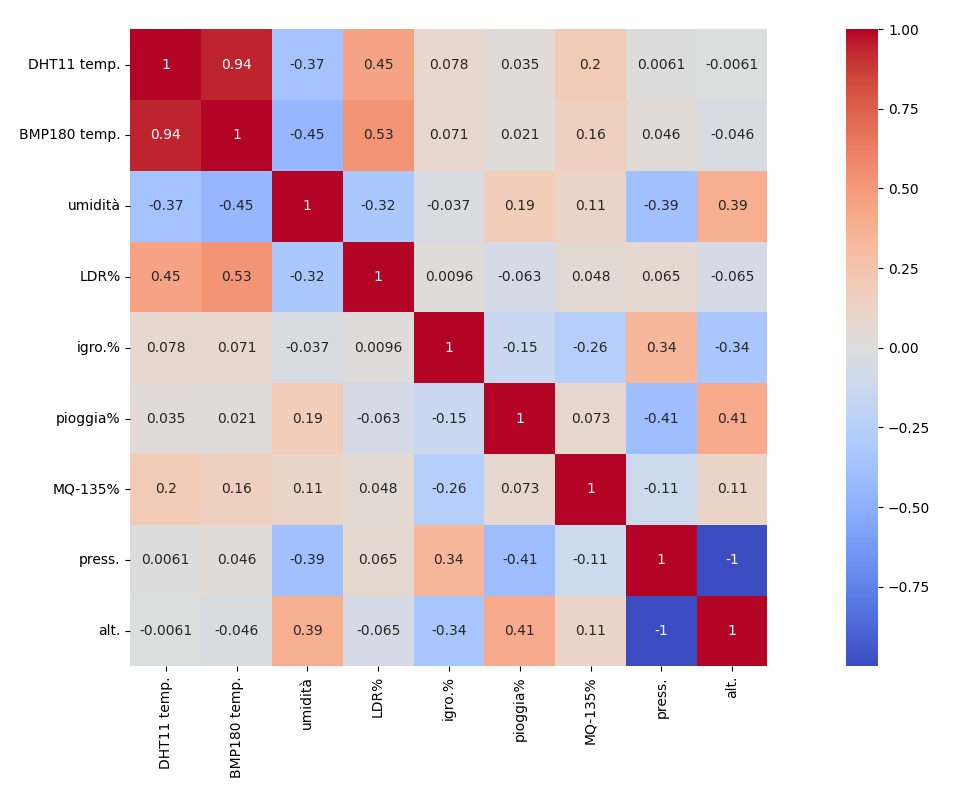
\includegraphics[scale=0.5]{assets/cov_matrix.png}
\caption{Matrice degli indici di correlazione di Pearson($\rho_p$)}
\label{fig:covariance}
\end{figure*}

La Figura \ref{fig:covariance} mostra una matrice ricavata calcolando gli indici di correlazione di Pearson($\rho_p$) per ogni sensore; ad ogni indice è stato assegnato un colore nella matrice
che va dal rosso, per una correlazione fortemente positiva, passando per il grigio, che indica nessuna particolare correlazione, fino al blu, per una correlazione fortemente negativa. Di seguito vediamo
alcuni valori particolarmente interessanti:

\begin{enumerate}
  \item la diagonale principale è tutta color rosso poiché ogni variabile è positivamente correlata con se stessa
  \item la correlazione fra le due temperature è fortemente positiva (0.97) misurando entrambe la stessa quantità
  \item la correlazione fra l'umidità e le due temperature è negativa (-0.37/-0.45), questo dipende da fattori fisici per cui, all'aumentare della temperatura l'aria si riscalda e ne consegue una diminuzione dell'umidità; 
  conseguentemente al diminuire della temperatura l'ambiente si raffredda e l'umidità aumenta
  \item la correlazione fra luminosità e temperatura è positiva (0.45/0.53), tenendo a mente che il valore di luminosità indica il giorno e la notte, all'aumentare della luminosità, ovvero durante il giorno, si ha un aumento
  della temperatura; al contrario la correlazione fra luminosità e umidità è negativa (-0.32), probabilmente questa non è da considerarsi veritiera poiché entrambe le variabili sono fortemente correlate alla temperatura e 
  questo valore ne è influenzato
  \item la pressione è fortemente correlata in maniera negativa con l'altitudine (-1), questo valore ci stupisce però è molto probabile che non sia corretto, infatti la pressione e l'altitudine sono calcolate
  entrambe dal sensore BMP180, in più vediamo che entrambe le variabili sono correlate all'umidità; è quindi probabile che la pressione sia correlata all'umidità, mentre l'altitudine è calcolata erroneamente sulla base 
  della pressione
\end{enumerate}

\section{Rilevazione anomalie}

Nelle sezioni precedenti abbiamo parlato della raccolta dei dati effettuata per 25 giorni consecutivi, inoltre abbiamo analizzato questi dati utilizzando i mezzi statistici; in questa sezione parliamo invece del passaggio 
successivo: il rilevamento delle anomalie. 

Per rilevare le anomalie si è deciso di addestrare un modello di Machine Learning utilizzando Edge Impulse\cite{edgeimpulse}, una piattaforma specializzata nella creazione di reti neurali ottimizzate per i dispositivi edge dell'IoT che
può essere utilizzata gratuitamente dai privati e le università. I dati raccolti sono stati scaricati localmente da InfluxBD in un file che, una volta processato, è stato ricaricato su Edge Impulse utilizzando le API di 
ingestion service\cite{eiapi}; nella sezione di "impulse design" si è creato un impulso utilizzando un blocco di pre-processing di tipo flatten, che calcola per ogni asse: valore massimo, 
minimo, deviazione standard e root mean square, ed infine un blocco di apprendimento di tipo K-means. Questo algoritmo è particolarmente utile poiché lavora creando dei cluster dai dati di training e rileva quelli anomali
calcolando la distanza del dato sospetto dai cluster, se è superiore ad una soglia viene ritenuta come anomala.
La rete neurale così creata è stata allenata utilizzando l'80\% dei dati raccolti, mentre il restante 20\% è stato utilizzato per la validazione. Addestrato il modello Edge Impulse consente di generare automaticamente
tutti i file necessari per l'utilizzo con Arduino, che sono poi importati come libreria esterna. Il rilevamento delle anomalie è stato fatto creando un programma chiamato `predictor.ino` che integra la funzione di raccolta 
dei dati di `collector.ino` con la libreria di anomaly detection creato prima; ogni 15 minuti l'ESP8266 si avvia leggendo i valori di ogni sensore ed usandoli per calcolare un "anomaly\_score" e caricando i valori di tutti i 
sensori su InfluxBD.

\begin{table*}[h!]
  \centering
  \begin{tabular}{ l l l l l }
    \hline
     & media & std & min & max \\
    \hline
    temperatura DHT11 & 2.81 & 4.70 & -3.0 & 18.0 \\
    temperatura BMP180 & 2.33 & 7.16 & -4.8 & 24.8 \\
    umidità & 86.03 & 3.14 & 64.0 & 91.0 \\
    LDR\% & 26.25 & 43.08 & 0.0 & 100.0 \\
    igrometro\% & 26.73 & 7.50 & 16.0 & 65.0 \\
    pioggia\% & 2.34 & 8.21 & 1.0 & 70.0 \\
    MQ-135\% & 7.87 & 0.47 & 3.0 & 8.0 \\
    pressione & 97320.60 & 294.61 & 96691.0 & 97898.0 \\
    altitudine & 339.67 & 25.26 & 290.17 & 393.59 \\
    \hline
  \end{tabular}
  \caption{Valori statistici ricavati dai dati anomali}
  \label{tab:anomalies}
\end{table*}

Il programma è stato eseguito per 7 giorni senza sosta, e al termine sono stati analizzati i dati raccolti ottenendo 734 campioni, di cui 455 anomalie (62\%) suddivise in 119(26\%) durante il giorno e 336(74\%) 
durante la notte. Nella Tabella \ref{tab:anomalies} sono mostrati alcuni valori statistici ricavati dai dati contenenti anomalie, in particolare notiamo come la temperatura minima sia di -3/-4.8, mentre la 
massima 18/24.8 e conseguentemente l'umidità minima e massima sia di 64 e 90.

\section{Conclusione}

Negli prossimi anni l'impiego della tecnologia avrà un ruolo fondamentale nella riduzione dell'impatto ecologico e nell'ottimizzazione di tutti i processi produttivi; in particolare nell'ambiente dell'agricoltura
si vede un enorme potenziale nell'unione di tutte le apparecchiature di monitoraggio presenti nelle grandi aziende con i concetti dell'Internet of Things. 

In questa relazione si è proposto lo sviluppo di una "Smart Box" IoT con lo scopo di raccogliere dati atmosferici da diversi sensori, calcolare le anomalie e segnalarle in un servizio situato sul cloud. 
Il lavoro si è svolto in 4 fasi: la progettazione e realizzazione dell'hardware, la raccolta di dati per un periodo di 25 giorni con lo scopo di addestrare un modello di Machine Learning volto al rilevamento delle 
anomalie, la creazione del suddetto modello e il suo utilizzo per la raccolta di dati anomali durante un periodo di 7 giorni. 
In aggiunta a queste fasi in questa relazione è stata proposta un'analisi statistica di base su tutti i dati raccolti in modo da comprendere meglio la loro composizione.

Fra i potenziali sviluppi futuri vi è la possibilità di gestire l'invio dei dati e delle anomalie senza avere la necessità di connettersi ad una rete WiFi, ad esempio utilizzando una smart card SIM dedicata oppure 
un ponte radio. Un altro ambito di miglioramento è l'aggiunta di sensori di diverso tipo, come ad esempio un anemometro per misurare la velocità del vento; inoltre è particolarmente interessante anche l'integrazione di 
più di una "Smart Box" IoT allo stesso tempo collocate in parti diverse dell'azienda con la possibilità di comunicazione fra di loro. 
Infine un aspetto da sviluppare ulteriormente è la durata della batteria, ottimizzando il power usage dei sensori o utilizzando direttamente delle batterie LiPo al posto di un power-bank.

\phantomsection
\printbibliography

\end{document}